\documentclass[fontsize=12bp, paper=a4]{scrarticle}
\usepackage[utf8]{inputenc}

\usepackage[english,main=serbian]{babel}
\usepackage[left=2cm, right=2cm, top=3cm, bottom=3cm]{geometry}
\usepackage[automark]{scrlayer-scrpage}
\usepackage{ragged2e}
\usepackage{amsmath}
\usepackage{mathabx}
\usepackage{hyperref}
\usepackage{graphicx}
\usepackage{wrapfig}
\usepackage{amssymb}
\usepackage{listings}
\usepackage{xcolor}
\usepackage{csquotes}
%\usepackage[backend=biber, style=numeric]{biblatex}

%
\definecolor{codegreen}{rgb}{0,0.6,0}
\definecolor{codegray}{rgb}{0.5,0.5,0.5}
\definecolor{codepurple}{rgb}{0.58,0,0.82}
\definecolor{backcolour}{rgb}{0.95,0.95,0.92}

\lstdefinestyle{mystyle}{
    backgroundcolor=\color{backcolour},   
    commentstyle=\color{codegreen},
    keywordstyle=\color{magenta},
    numberstyle=\tiny\color{codegray},
    stringstyle=\color{codepurple},
    basicstyle=\ttfamily\footnotesize,
    breakatwhitespace=false,         
    breaklines=true,                 
    captionpos=b,                    
    keepspaces=true,                 
    numbers=left,                    
    numbersep=5pt,                  
    showspaces=false,                
    showstringspaces=false,
    showtabs=false,                  
    tabsize=2
}

\lstset{style=mystyle}

\renewcommand\lstlistingname{Implementacija}
\renewcommand\lstlistlistingname{Implementacija}

%

\graphicspath{ {./images/} }

%
\title{Seminarski rad} 
\subtitle{iz predmeta Teorijske osnove veštačke inteligencije}

\begin{document}

\begin{titlepage}
    \vspace{\stretch{1}}
    
    \begin{center}
        
        \vspace*{8cm}
        
        \large{Univerzitet u Kragujevcu}
        
        \vspace*{1cm}

        {\bfseries \LARGE Domaći zadatak}
        
        \large{iz predmeta Sistem za podršku odlučivanju}
        
        \vspace*{1cm}
        \large{Tema:}

        \Large{Implementacija regresionih algoritmima nadgledanog učenja}


        \vspace*{2cm}
    \end{center}
    \hfill{\parbox[s]{8cm}{

    mentori: 
    \begin{tabular}{l}
        \\
        \\
        Ognjen Pavić, \\
        prof. dr. Tijana Geroski, \\
        prof. dr. Nenad Filipović 
    \end{tabular}
    
    student: \begin{tabular}{l}
        Željko Simić 3vi/2023
    \end{tabular}
    }}

    \hspace*{\fill} 

    \vspace*{2cm}

    \begin{center}
        Kragujevac 2024.
    \end{center}
\end{titlepage}


\setcounter{page}{1}
\justifying
\linespread{0.9}
\cfoot[\pagemark]{\pagemark}
\ofoot[]{}
\ohead[]{Željko Simić 3vi/2023}
\chead[]{}
\ihead[]{Univerzitet u Kragujevcu}
%
\justifying

\section{Uvod}

Dat je \verb|``housing.csv''| dataset.\cite{dataset} Namenjen za sagledanje procene vrednosti kuće. U sebi sadr\i 20640 instanci (uzoraka), a ima u sebi za svaki po 9 kolona atributa (posmatran kao ulazna vrednost):
\begin{itemize}
    % \item \verb|User ID| - Ukazuje na udeljeni jedinstveni identifikator korisnika posmatranog sistema. \textbf{Biće izbačen pri sagledanju i neće biti uzet u obzir};
    % \item \verb|Gender| - Ukazuje na pol korisnika, kategoričkih vrednosti (\verb|Male, Female|);
    % \item \verb|Age| - Ukazuje na starost korisnika, sa kontinualnim vrednostima u domenu $[18,60]$
    
    \item \verb|longitude| - ugao zastupljene lokacije naspram zapada (većom vrednošću on je dalje) i ekvatora planete Zemlje, $[-180, 180]$;
    \item \verb|latitude| - ugao zastupljene lokacije naspram severa (većom vrednošću on je dalje) i meridijana planete Zemlje $[-180, 180]$;
    \item \verb|housing_median_age| - stopa osrednje godine kuće, kontinualna vrednost;
    \item \verb|total_rooms| - ukupan broj soba, numerička vrednost;
    \item \verb|total_bedrooms| - ukupan broj spavaćih soba, numerička vrednost;
    \item \verb|population| - broj ljudi u naselju, numerička vrednost;
    \item \verb|households| - broj domaćinstava u naselju, numerička vrednost;
    \item \verb|median_income| - stopa osrednjeg prihoda u  naselju, numerička vrednost;
    \item \verb|ocean_proximity| - udaljenost lokacije od najbliže lokacije mora, kategorička vrednost.
\end{itemize}
i 1 ciljnu vrednost (posmatran kao izlaznu vrednost):
\begin{itemize}
    \item \verb|median_house_value| - stopa osrednjeg vrednovanja kuće u USD valuti;
\end{itemize}

\newpage
\section{Metodologija}


% korelacija ulaza naspram izlaza

% distribucija po starosti koji nisu / jesu kupili 
% distribucija po plaćenosti koji nisu / jesu kupili 


Uz tekst seminarskog rada je priložen izvorni kod (na putanji \verb|./src/main.py|) koji će se ovde sagledati. Implementacija 1. u sebi sadrži deklaracije uvedenih modula iz kojih će biti pozivane njihove komponente u daljem radu (praktično realizovanje teorijskog rada na ovu temu\cite{mojRad}). Korišćen je objektni tip podataka \verb|pandas.DataFrame|\cite{pandasDF} kojim će biti urađeno strukturno skladištenje (sa metodom \verb|pd.read_csv(putanja_csv_fajla_skupa_podataka)|) i manipulisano elementima skupa podataka koji je bio pomenut u uvodu. Biće izvršeno zaobilaženje prikaza obaveštenja na standardnom izlazu greške, predprocesiranje u kom spada eliminisanje nedostajućih instanci, pokušaj eliminacije duplikata, enkodiranje \verb|ocean_proximity| atributa (da bi bio prikladan za dalji rad sa regresijom iz vrednosti tipa string-a u broj)\cite{labelEncoding}, skaliranje vrednosti features-a \verb|MinMaxScaler|-om (po pretpostavci da nam normalna distribucija, uglavnom, nije zastupljena i obavljena je zarad skupljanja svih vrednosti na gomilu u početnoj oblasti $[0,1]$)\cite{scaleDist}, podela skupa podataka uz \verb|train_test_split(...)| na trening i test skupove podataka po nekoj razmeri $8:2$ za ulazne i izlazne vrednosti klasifikacija.\cite{train_test_split}


\begin{lstlisting}[language=Python, caption=Predprocesiranje podataka i navođenje modula koji će se koristiti]

import pandas as pd
import seaborn as sns
import matplotlib.pyplot as plt
import numpy as np
from sklearn.preprocessing import LabelEncoder
from sklearn.preprocessing import MinMaxScaler
from sklearn.model_selection import train_test_split, GridSearchCV
from sklearn.linear_model import LinearRegression
from sklearn.preprocessing import PolynomialFeatures
from sklearn.tree import DecisionTreeRegressor
from sklearn.ensemble import RandomForestRegressor

from sklearn.svm import SVR
from sklearn.metrics import r2_score
import warnings 
warnings.filterwarnings("ignore")

...
dataframe = pd.read_csv('./housing.csv')
print("==================")
print("Nedostajuce vrednosti:")
print(dataframe.isnull().sum())
df1 = dataframe[dataframe['total_bedrooms'].notnull()]

print("==================")
duplikati = df1[df1.duplicated()]
if len(duplikati) == 0:
	print("Nema duplikata")
else:
	print(duplikati)
print("==================")	

df1['ocean_proximity']= LabelEncoder().fit_transform(df1['ocean_proximity']) 
...
y1 = df1['median_house_value']
x1 = df1[["longitude","latitude","housing_median_age","total_rooms","total_bedrooms","population","households","median_income","ocean_proximity"]]
sc = MinMaxScaler()
x1_scalled = sc.fit_transform(x1)


X_train, X_test, y_train, y_test = train_test_split(x1_scalled, y1, test_size = 0.2)
\end{lstlisting}

Na izlazu 1. je prikazano da 207 instanci ima nedostajuće vrednosti i oni će biti eliminisani nadalje, a takođe je prikazano da duplikata nije takođe bilo. 

\renewcommand\lstlistingname{Izlaz}
\renewcommand\lstlistlistingname{Izlaz}
\setcounter{lstlisting}{0}
\begin{lstlisting}[caption=Nedostajuće vrednosti i duplikati]
==================
Nedostajuce vrednosti:
longitude               0
latitude                0
housing_median_age      0
total_rooms             0
total_bedrooms        207
population              0
households              0
median_income           0
median_house_value      0
ocean_proximity         0
dtype: int64
==================
Nema duplikata
==================
\end{lstlisting}

\vbox{}

\vbox{}

U implementaciji 2. vrši se generisanje slika 1. (za korelaciju među features-ima po verovatonosnoj distributivnoj funkciji (PDF) na target vrednost \verb|Purchased|), 2. (za distribuciju naspram feature-a \verb|Age| i target vrednosti), 3. (za distribuciju naspram feature-a \verb|EstimatedSalary|). Ovo sve je obavljeno uz metode \verb|seaborn.pairplot| za sliku 1.\cite{pairplot} i \verb|seaborn.displot| za slike 2. i 3.\cite{displot}

\renewcommand\lstlistingname{Implementacija}
\renewcommand\lstlistlistingname{Implementacija}
\setcounter{lstlisting}{1}
\begin{lstlisting}[language=Python, caption=Navođenje načina vizuelizacija za sliku \texttt{1.}]
sns.pairplot(dataframe, palette="Spectral", hue="median_house_value", dropna=True)
plt.show()
\end{lstlisting}

Ovaj deo koji sledi važi samo za vrednosti koje još uvek nisu skalirane maločas pomenutim postupkom skaliranja.

Na slici 1. je moguće uočiti da PDF za feature \verb*|longitude| \verb*|median_house_value| vrednosti ukazuje na zastupljenost po toj komponenti lokacije na domenu [-125, -122] i [-120, -106] najviše za osrednju vrednost kuće od 500000\$.

Za PDF \verb*|longitude| naspram \verb*|latitude| po \verb|median_house_value| može se videti zastupljenost [-116, -114] naspram [30,35] i [-124, -120] naspram [40, 45] za 300000\$ i naniže, a za više osrednje vrednosti kuće na [-122, -114] naspram [30,35].

Za PDF \verb*|longitude| naspram \verb*|house_median_age| po \verb|median_house_value| može se videti zastupljenost [-116, -114] naspram [0,75] i [-124, -120] naspram [0, 75] za 300000\$ i naniže, a za više osrednje vrednosti kuće na [-122, -116] naspram [0,75].


Za PDF \verb*|longitude| naspram \verb*|total_rooms| po \verb|median_house_value| može se videti zastupljenost [-116, -114] naspram [0,25000] i [-124, -120] naspram [0, 25000] za 300000\$ i naniže, a za više osrednje vrednosti kuće na [-122, -116] naspram [0,25000].

Za PDF \verb*|longitude| naspram \verb*|total_bedrooms| po \verb|median_house_value|  može se videti zastupljenost [-116, -114] naspram [0,25000] i [-124, -120] naspram [0, 5000] za 300000\$ i naniže, a za više osrednje vrednosti kuće na [-122, -116] naspram [0,5000].

Za PDF \verb*|longitude| naspram \verb*|population| po \verb|median_house_value| može se videti zastupljenost [-116, -114] naspram [0,10000] i [-124, -120] naspram [0,10000] za 300000\$ i naniže, a za više osrednje vrednosti kuće na [-122, -114] naspram [0,10000].

Za PDF \verb*|longitude| naspram \verb*|households| po \verb|median_house_value| može se videti zastupljenost [-116, -114] naspram [0,1000] i [-124, -120] naspram [0,1000] za 300000\$ i naniže, a za više osrednje vrednosti kuće na [-122, -114] naspram [0,5000].

Za PDF \verb*|longitude| naspram \verb*|median_income| po \verb|median_house_value| može se videti zastupljenost [-116, -114] naspram [30,35] i [-124, -120] naspram [0, 10] za 300000\$ i naniže, a za više osrednje vrednosti kuće na [-122, -114] naspram [0,10], osim za 500000\$ na [-119, -116] naspram [10, 20].

PDF za \verb*|latitude| \verb*|median_house_value| vrednosti ukazuje na zastupljenost po toj komponenti lokacije na domenu [32, 34] i [36,38] naniže za osrednju vrednost kuće od 500000\$.

Za PDF \verb*|latitude| naspram \verb*|house_median_age| po \verb|median_house_value| može se videti zastupljenost [38, 42] naspram [0, 50] za 300000\$ i naniže.

Za PDF \verb*|latitude| naspram \verb*|total_rooms| po \verb|median_house_value| može se videti zastupljenost [38, 42] naspram [0,10000] za 300000\$ i naniže.

Za PDF \verb*|latitude| naspram \verb*|total_bedrooms| po \verb|median_house_value| može se videti zastupljenost [38, 42] naspram [0,2000] za 300000\$ i naniže.

Za PDF \verb*|latitude| naspram \verb*|population| po \verb|median_house_value| može se videti zastupljenost [38, 42] naspram [0,10000] za 300000\$ i naniže.

Za PDF \verb*|latitude| naspram \verb*|households| po \verb|median_house_value| može se videti zastupljenost [38, 42] naspram [0,2000] za 300000\$ i naniže.

Za PDF \verb*|latitude| naspram \verb*|median_income| po \verb|median_house_value| može se videti zastupljenost [38, 42] naspram [0,10] za 300000\$ i naniže, a za 500000\$ [37, 38] naspram [10,15] i [33,35] naspram [10,15].

PDF za \verb*|house_median_age| \verb*|median_house_value| vrednosti ukazuje na zastupljenost po toj komponenti lokacije na domenu [0, 50] naniže za osrednju vrednost kuće od 500000\$.
 
Za PDF \verb*|house_median_age| naspram \verb*|total_rooms| po \verb|median_house_value| može se videti zastupljenost [0, 40] naspram [0, 10000] za 300000\$ i naniže.

Za PDF \verb*|house_median_age| naspram \verb*|total_bedrooms| po \verb|median_house_value| može se videti zastupljenost [10, 50] naspram [0, 2000]   za 300000\$ i naniže.

Za PDF \verb*|house_median_age| naspram \verb*|population| po \verb|median_house_value| može se videti zastupljenost [5,50] naspram [0, 5000]  za 300000\$ i naniže.

Za PDF \verb*|house_median_age| naspram \verb*|households| po \verb|median_house_value| može se videti zastupljenost [5, 50] naspram [38, 42] za 300000\$ i naniže.

Za PDF \verb*|house_median_age| naspram \verb*|median_income| po \verb|median_house_value| može se videti zastupljenost [0, 50] naspram [0, 10] za 300000\$ i naniže, a za 500000\$ na [10,20] naspram [0, 50].

PDF za \verb*|total_rooms| \verb*|median_house_value| vrednosti ukazuje na zastupljenost po toj komponenti lokacije na domenu [0, 10000] najviše za osrednju vrednost kuće od 400000\$, pa za sve ostale u tom sličnom domenu.

Za PDF \verb*|total_rooms| naspram \verb*|total_bedrooms| po \verb|median_house_value| može se videti zastupljenost [0, 10000] naspram [0, 2000] za 300000\$ i naniže.

Za PDF \verb*|total_rooms| naspram \verb*|population| po \verb|median_house_value| može se videti zastupljenost [0, 10000] naspram [0, 10000] za 300000\$ i naniže.

Za PDF \verb*|total_rooms| naspram \verb*|households| po \verb|median_house_value| može se videti zastupljenost [0, 10000] naspram [0, 2000] za 300000\$ i naniže.

Za PDF \verb*|total_rooms| naspram \verb*|median_income| po \verb|median_house_value| može se videti zastupljenost [0, 20000] naspram [0, 5] za 300000\$ i naniže, a za 500000\$ na [0,10000] naspram [10, 20].

PDF za \verb*|total_bedrooms| \verb*|median_house_value| vrednosti ukazuje na zastupljenost po toj komponenti lokacije na domenu [0, 1000] najviše za osrednju vrednost kuće od 500000\$, pa za sve ostale u tom sličnom domenu.

Za PDF \verb*|total_bedrooms| naspram \verb*|population| po \verb|median_house_value| može se videti zastupljenost [0, 5000] naspram [0, 10000] za 300000\$ i naniže.

Za PDF \verb*|total_bedrooms| naspram \verb*|households| po \verb|median_house_value| može se videti zastupljenost [0, 5000] naspram [0, 5000] za 300000\$ i naniže.

Za PDF \verb*|total_bedrooms| naspram \verb*|median_income| po \verb|median_house_value| može se videti zastupljenost [0, 5000] naspram [0, 5] za 300000\$ i naniže, a za 500000\$ na [0,2000] naspram [10, 18].

PDF za \verb*|population| \verb*|median_house_value| vrednosti ukazuje na zastupljenost po toj komponenti lokacije na domenu [0, 5000] najviše za osrednju vrednost kuće od 500000\$, pa za sve ostale u tom sličnom domenu.

Za PDF \verb*|population| naspram \verb*|households| po \verb|median_house_value| može se videti zastupljenost [0, 5000] naspram [0, 5000] za 300000\$ i naniže, a za 500000\$ na [0,2000] naspram [10, 18].

Za PDF \verb*|population| naspram \verb*|median_income| po \verb|median_house_value| može se videti zastupljenost [0, 5000] naspram [0, 5] za 300000\$ i naniže, a za 500000\$ na [0,2000] naspram [10, 18].

PDF za \verb*|households| \verb*|median_house_value| vrednosti ukazuje na zastupljenost po toj komponenti lokacije na domenu [0, 5000] najviše za osrednju vrednost kuće od 500000\$, pa za sve ostale u tom sličnom domenu.

Za PDF \verb*|households| naspram \verb*|median_income| po \verb|median_house_value| može se videti zastupljenost [0, 4000] naspram [0, 5] za 300000\$ i naniže, a za 500000\$ na [0,2000] naspram [10, 18].

PDF za \verb*|median_income| \verb*|median_house_value| vrednosti ukazuje na zastupljenost po toj komponenti lokacije na domenu [0, 2] za osrednju vrednost kuće od 500000\$, a na domenu [10,15] najviše za osrednju vrednost kuće od 100000\$, pa za sve ostale u tom sličnom domenu.


\begin{figure}[h!]
    \centering
    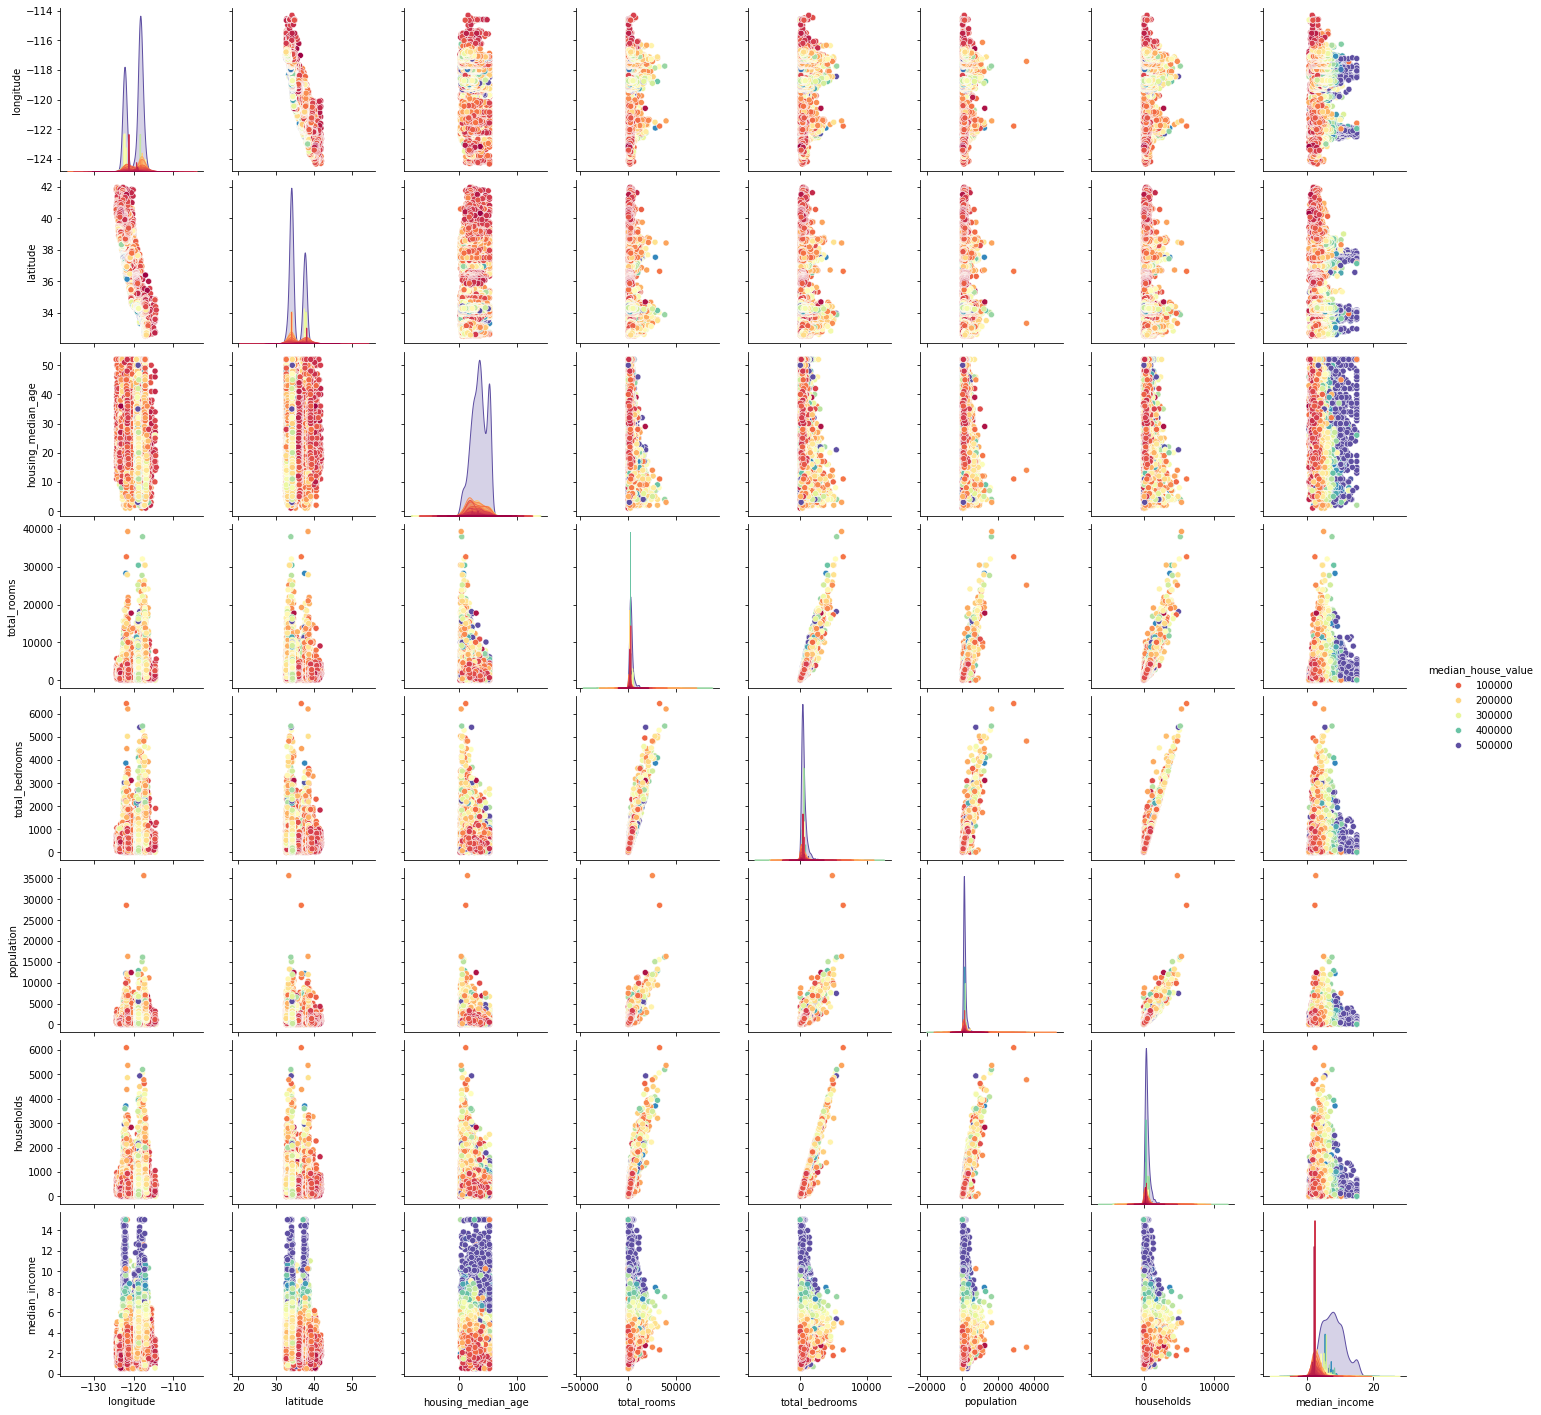
\includegraphics[width=1\textwidth]{1.png}
    \caption{\centering Vizuelizacija za korelaciju među features-ima po verovatonosnoj distributivnoj funkciji (PDF) na target vrednost \texttt{median\_house\_value}}
\end{figure}      


\newpage
\vbox{}
\vbox{}
\vbox{}
\vbox{}
\vbox{}
\vbox{}
\vbox{}

\section{Metodologija}

U implementaciji 3. dat je postupak ispisa evaluacije (korena) središnje kvadratne greške koji će se prikazivati. Ova funkcija će se nadalje primenjivati u daljem radu, uglavnom, a pritom će se prikazivati \textit{R2 score}.

\renewcommand\lstlistingname{Implementacija}
\renewcommand\lstlistlistingname{Implementacija}
\setcounter{lstlisting}{2}

\begin{lstlisting}[language=Python, caption=Postupak ispisa evaluacije (korena) središnje kvadratne greške]
def evaluate(y_pred, y_test,name):

    square_error=np.array(y_test-y_pred)
    square_error=np.power(square_error,2)
    square_error=np.sum(square_error)

    mean_square_error=square_error/len(y_pred)

    root_mean_square_error=np.sqrt(mean_square_error)

    print(name)
    print('mean square error: ' + str(round(mean_square_error,2)))
    print('root mean square error: ' + str(round(root_mean_square_error,2)))
    print()

    return mean_square_error,root_mean_square_error

\end{lstlisting}

\subsection{Jednostavna linearna regresija (SLR)}

Vršiće se treniranja i predikcije naspram svakog feature-a ponaosob, pošto ovaj algoritam\cite{LR} radi sa samo 1 feature-om, a takođe ovaj algoritam nema nikakvih hiperparametara.

U ovom slučaju u implementaciji 4. radi se evaluacija naspram feature-a, usresređujući se na ciljnu vrednost, za svaku je ispisan kranji MSE i RMSE. Moguće je uočiti da je dat najviše značaj treniranju i predikciji nad feature-om \texttt{median\_income}. Za taj feature dat je i R2 score i iscrtan grafik za pravu regresije među instancama, uzimanjem dveju tačaka naspram koordinate najmanjeg ulaznog parametara i njegovom multiplikacijom odnosa $1.01$, pravljenja niza od 10 elemenata i formiranjem niza y elemenata prema nagibu i odsečkom na y-osi.

\begin{lstlisting}[language=Python, caption=Postupak evaluacija naspram svakog feature-a ponaosob.]
model = LinearRegression()

model.fit(X_train[:,0].reshape(-1,1),y_train)
predicted = model.predict(X_test[:,0].reshape(-1,1))

mse,rmse=evaluate(predicted, list(y_test), "Simple linear regresion over longitude")
########################################
model.fit(X_train[:,1].reshape(-1,1),y_train)
predicted = model.predict(X_test[:,1].reshape(-1,1))

mse,rmse=evaluate(predicted, list(y_test), "Simple linear regresion over latitude")
########################################
model.fit(X_train[:,2].reshape(-1,1),y_train)
predicted = model.predict(X_test[:,2].reshape(-1,1))

mse,rmse=evaluate(predicted, list(y_test), "Simple linear regresion over housing_median_age")
########################################
model.fit(X_train[:,3].reshape(-1,1),y_train)
predicted = model.predict(X_test[:,3].reshape(-1,1))

mse,rmse=evaluate(predicted, list(y_test), "Simple linear regresion over total_rooms")
########################################
model.fit(X_train[:,4].reshape(-1,1),y_train)
predicted = model.predict(X_test[:,4].reshape(-1,1))

mse,rmse=evaluate(predicted, list(y_test), "Simple linear regresion over total_bedrooms")
########################################
model.fit(X_train[:,5].reshape(-1,1),y_train)
predicted = model.predict(X_test[:,5].reshape(-1,1))

mse,rmse=evaluate(predicted, list(y_test), "Simple linear regresion over population")
########################################
model.fit(X_train[:,6].reshape(-1,1),y_train)
predicted = model.predict(X_test[:,6].reshape(-1,1))

mse,rmse=evaluate(predicted, list(y_test), "Simple linear regresion over households")
########################################
model.fit(X_train[:,7].reshape(-1,1),y_train)
predicted = model.predict(X_test[:,7].reshape(-1,1))

mse,rmse=evaluate(predicted, list(y_test), "Simple linear regresion over median_income")

print(f"R2 score: {r2_score(y_test, predicted)}")
plt.figure()
plt.title('regression visualisation')
plt.scatter(X_test[:,7], y_test, color='black')
plt.plot(X_test[:,7], predicted)
plt.show()

plt.figure()
plt.title('linear model visualisation')
plt.scatter(X_test[:,7], y_test, color='black')
coefficients = model.coef_
intercept = model.intercept_
k = coefficients
n = intercept

line_x = np.arange(min(X_train[:,7]), 1.01*max(X_train[:,7]), (max(X_train[:,7])- min(X_train[:,7]))/10)
line_y = k * line_x + n
plt.plot(line_x, line_y, color='red')
plt.show()
########################################
model.fit(X_train[:,8].reshape(-1,1),y_train)
predicted = model.predict(X_test[:,8].reshape(-1,1))

mse,rmse=evaluate(predicted, list(y_test), "Simple linear regresion over ocean_proximity")
\end{lstlisting}

\subsection{Višestruka linearna regresija (MLR)}

Vrši se instanciranje klase modula \verb|LinearRegression|, vrši se obuka nad trening skupom, ispisuju ste statistike greške MSE, RMSE, R2 score i iscrtava se grafik linearne regresije kao i ranije. Hiperparametara kod ovog algoritma nema.

\begin{lstlisting}[language=Python, caption=Postupak MLR-a]
model = LinearRegression()
model.fit(X_train,y_train)
predicted = model.predict(X_test)

mse,rmse=evaluate(predicted, list(y_test), "Multiple linear regresion")
print(f"R2 score: {r2_score(y_test, predicted)}")

plt.figure()
plt.title('linear model visualisation')
plt.scatter(X_test, y_test, color='black')
coefficients = model.coef_
intercept = model.intercept_
k = coefficients
n = intercept

line_x = np.arange(min(X_train), 1.01*max(X_train), (max(X_train)- min(X_train))/10)
line_y = k * line_x + n
plt.plot(line_x, line_y, color='red')
plt.show()
\end{lstlisting}

\subsection{Polinomijalna linearna regresija (PLR)}

\verb|PolynomialFeatures|\cite{plr} u kombinaciji sa \verb|LinearRegression|. Korišćen je algoritam za usklađivanje za rad sa polinomijalnim linearnim regresijama. Postavljen je inicijalni stepen polinoma koji će izgraditi aproksimiranu krivu za ulazne vrednosti trening skupa koji će biti prilagođeni da rade nad takvim tipom algoritma. Formira se niz tačaka za grafik na koji će se iscrtati kriva i tačke instanci koje će biti razdvojene tom krivom. Predikcijom dobijaju se koeficijenti elemenata svakog stepena polinoma, generiše se isti niz kao za pravu za ulazne vrednosti (prvog feature-a) trening skupa, a zatim se formira novi nizovi gde su svi elementi stepenovani na kvadratni i kubni stepen. Takođe je uzet u obzir odsečak sa y-osom. 
Ovde je uzet u obzir \verb|households| feautre kao prikaz instanci, koji po mom mišljenju ima doličan prikaz razdvajanja.


\begin{lstlisting}[language=Python, caption=Postupak PLR-a]
polynomialRegression = PolynomialFeatures(degree = 3)
X_train_poly = polynomialRegression.fit_transform(X_train)
X_test_poly = polynomialRegression.transform(X_test)
model = LinearRegression()
model.fit(X_train_poly, y_train)

predicted = model.predict(X_test_poly)

mse, rmse = evaluate(list(y_test), predicted, 'polynomial_regression')
print(f"R2 score: {r2_score(y_test, predicted)}")
    
plt.figure()
plt.title('polynomial regr visualization')
plt.scatter (X_test[:,6], y_test, color="black")

coefficients = model.coef_
intercept = model.intercept_
k1 = coefficients[0]
k2 = coefficients[1]
k3 = coefficients[2]
n = intercept

X = X_train[:,0]
line_x1 = np.arange(min(X), 
 					max(X) * 1.01, 
 					(max(X) - min(X)) / 10)
line_x2 = line_x1 ** 2
line_x3 = line_x1 ** 3

line_y3 = k1*line_x1 + k2*line_x2 + k3*line_x3 + n

plt.plot(line_x1, line_y3, color="red")
plt.show()
\end{lstlisting}

\subsection{Regresija stabla odlučivanja}

Postupak regresije stabla odlučivanja\cite{DTR} bez i sa optimizacijom hiperparametrima je obavljen obukom nad trening skupom podataka, kao i predikcijom nad test skupom podataka, ispisan je takođe MSE, RMSE, R2 score. Korišćeni hiperparametri su:
\begin{itemize}
    \item \verb|splitter| - koji je implicitno postavljen na vrednost best i naznačava strategiju kojom će se vršiti podele grananjima;
    \item \verb|max_depth| - koji implicitno nema nikakvu vrednost, ističe se kolika je dubina stabla koje se generiše;
    \item \verb|min_samples_leaf| - implicitna vrednost mu je 1, a označava koliko mora najmanje instanci sadržati čvor lista stabla;
    \item \verb|min_weight_fraction_leaf| - implicitna vrednost 0, a označava minimalno nephodnu sumu težina svih uzoraka u listu stabla; 
    \item \verb|max_features| - implicitno nema kriterijuma, ali kad ima njime se zaključuje na koiji način, kojom funkcijom će se sagledati podela naspram broja feature vrednosti.
    \item \verb|max_leaf_nodes| - implicitno nema postavljen zahtevajući kriterijum što naznačava da je ograničenje broja čvorova $\infty$, a rast stabla će se obavljati u najbolji-prvo maniru.
\end{itemize}

Optimizacija hiperparametrima\cite{GridSearchCV} će se obaviti i nakon svake evaluacije algoritmom istaći će se najbolji ishodujući model sa njegovim hiperparametrima. Takođe je obavljen stratifikovan cross-validation postupak.

\begin{lstlisting}[language=Python, caption=\centering Postupak regresije stabla odlučivanja bez i sa optimizacijom hiperparametrima]
decisionTreeRegressor=DecisionTreeRegressor()
decisionTreeRegressor.fit(X_train, y_train)
predicted = decisionTreeRegressor.predict(X_test)
mse, rmse = evaluate(list(y_test), predicted, 'decision tree')
print(f"R2 score: {r2_score(y_test, predicted)}")

print("------------------")
# https://www.nbshare.io/notebook/312837011/Decision-Tree-Regression-With-Hyper-Parameter-Tuning-In-Python/
params={"splitter":["best","random"],
            "max_depth" : [1,3,5,7,9,11,12],
            "min_samples_leaf":[1,2,3,4,5,6,7,8,9,10],
            "min_weight_fraction_leaf":[0.1,0.2,0.3,0.4,0.5,0.6,0.7,0.8,0.9],
            "max_features":["auto","log2","sqrt",None],
            "max_leaf_nodes":[None,10,20,30,40,50,60,70,80,90]}

modelGrid=GridSearchCV(DecisionTreeRegressor(),param_grid=params,cv=5)
modelGrid.fit(X_train,y_train)
modelBest = modelGrid.best_estimator_
predicted=modelBest.predict(X_test)
mse,rmse=evaluate(predicted, list(y_test), "decision tree with hyperparameter optimization")
print(f"R2 score: {r2_score(y_test, predicted)}")
print('best params after grid search: ')
print(modelGrid.best_params_)

\end{lstlisting}

\subsection{Regresija slučajne šume}
Postupak regresije slučajnih šuma\cite{RFR} bez i sa optimizacijom hiperparametrima je obavljen obukom nad trening skupom podataka, kao i predikcijom nad test skupom podataka, ispisan je takođe MSE, RMSE, R2 score. Korišćeni hiperparametri su: \texttt{n\_estimators} (naznačava koji broj stabala odlučivanja će se uzeti u obzir, implicitno se uzima njih 100), \texttt{max\_features}, \texttt{max\_depth}, \texttt{max\_leaf\_nodes} (isto značenje kao i kod stabala odlučivanja).

Optimizacija hiperparametrima je obavljena na sličan način kao i kod stabala odlučivanja.
\begin{lstlisting}[language=Python, caption=\centering Postupak slučajnih šuma bez i sa optimizacijom hiperparametrima]
randomForestRegressor=RandomForestRegressor(n_estimators=10,random_state=0)
randomForestRegressor.fit(X_train, y_train)
predicted = randomForestRegressor.predict(X_test)
mse, rmse = evaluate(list(y_test), predicted, 'random forest')
print(f"R2 score: {r2_score(y_test, predicted)}")
print("------------------")
# https://www.geeksforgeeks.org/random-forest-hyperparameter-tuning-in-python/
params={'n_estimators': [25, 50, 100, 150], 
    'max_features': ['sqrt', 'log2', None], 
    'max_depth': [3, 6, 9], 
    'max_leaf_nodes': [3, 6, 9]
 	}
            
modelGrid=GridSearchCV(RandomForestRegressor(),param_grid=params,cv=5)
modelGrid.fit(X_train,y_train)
modelBest = modelGrid.best_estimator_
predicted=modelBest.predict(X_test)
mse,rmse=evaluate(predicted, list(y_test), "Random Forest with hyperparameter optimization")
print(f"R2 score: {r2_score(y_test, predicted)}")
print('best params after grid search: ')
print(modelGrid.best_params_)
\end{lstlisting}


\subsection{Regresija potpornim vektorima (SVR)}

Postupak regresije metoda potpornih vektora (SVR)\cite{SVR} bez i sa optimizacijom hiperparametrima je obavljen obukom nad trening skupom podataka, kao i predikcijom nad test skupom podataka, ispisan je takođe MSE, RMSE, R2 score. Korišćeni hiperparametri su: 
\begin{itemize}
    \item \verb|C| - implicitno je postavljeno na vrednost 0, a ovo je parametar regularizacije - naznačava jačinu regularizacije inverzno proporcionalno, a ona mora biti striktno pozitivna;
    \item \verb|gamma| - implicitno je \verb|'scale'|, primenjena je pri režimima kernela \verb|'rbf', 'poly', 'sigmoid'|;
    \item \verb|kernel| - implicitno \verb|'rbf'| režim se uzima u obzir, ovim parametrom se uzima u obzir režim kernela kojim će baratati algoritam.
\end{itemize}
Optimizacija hiperparametrima je obavljena na sličan način kao i kod stabala odlučivanja.
\begin{lstlisting}[language=Python, caption=\centering Postupak regresije metoda potpornih vektora (SVR) bez i sa optimizacijom hiperparametrima]
supportVectorRegressor=SVR(kernel='rbf')
supportVectorRegressor.fit(X_train,y_train)
predicted = supportVectorRegressor.predict(X_test)
mse, rmse = evaluate(list(y_test), predicted, 'svr')
print(f"R2 score: {r2_score(y_test, predicted)}")
print("------------------")
# https://www.geeksforgeeks.org/random-forest-hyperparameter-tuning-in-python/
params = {'C': [0.1, 10, 100],  
              'gamma': [1, 0.01, 0.001], 
              'kernel': ['linear', 'poly', 'rbf', 'sigmoid']}  


modelGrid=GridSearchCV(SVR(),param_grid=params,cv=5)
modelGrid.fit(X_train,y_train)
modelBest = modelGrid.best_estimator_
predicted=modelBest.predict(X_test)
mse,rmse=evaluate(predicted, list(y_test), "Support vector regression with hyperparameter optimization")
print(f"R2 score: {r2_score(y_test, predicted)}")
print('best params after grid search: ')
print(modelGrid.best_params_)
\end{lstlisting}

\newpage
\renewcommand\lstlistingname{Izlaz}
\renewcommand\lstlistlistingname{Izlaz}
\setcounter{lstlisting}{1}

\section{Rezultati}
\subsection{Jednostavna linearna regresija (SLR)}
U izlazu 2. moguće je uočiti da je najbolji ishod regresije bio nad feature-om \verb|median_income| sa MSE: $7274334668.63$ i RMSE od $85289.71$, dok R2 score za njega samo sračunat je bio oko $0.46$.
\begin{lstlisting}[caption=\centering SLR za sve features-e ponaosob]
Simple linear regresion over longitude
mean square error: 13249925560.75
root mean square error: 115108.32


Simple linear regresion over latitude
mean square error: 13054128998.76
root mean square error: 114254.67


Simple linear regresion over housing_median_age
mean square error: 13151138804.24
root mean square error: 114678.41


Simple linear regresion over total_rooms
mean square error: 13116182951.67
root mean square error: 114525.91


Simple linear regresion over total_bedrooms
mean square error: 13268375872.85
root mean square error: 115188.44


Simple linear regresion over population
mean square error: 13289199266.77
root mean square error: 115278.79


Simple linear regresion over households
mean square error: 13244660307.41
root mean square error: 115085.45


Simple linear regresion over median_income
mean square error: 7274334668.63
root mean square error: 85289.71
R2 score: 0.45277738375262455
\end{lstlisting}

Data je slika 2. na kojoj je prikazan postupak regresije nad feature-om \verb|median_income|.

%%% fali slika

\begin{figure}[h!]
    \centering
    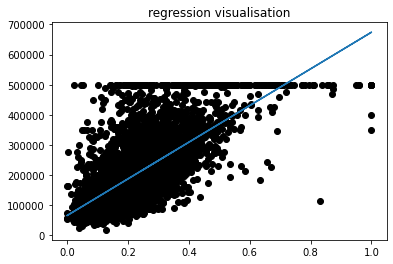
\includegraphics[width=0.5\textwidth]{2.png}
    \caption{\centering Jednostavna linearna regresija nad feature-om \texttt{median\_income}}
\end{figure}      


\subsection{Višestruka linearna regresija (MLR)}
Dobijen ispis na izlaz 3. za primenjen algoritam MLR modela je takav da mu je MSE: $5180413707.33$, RMSE: $71975.09$, R2 score: ~$0.61$.
\begin{lstlisting}[caption=\centering MLR]
Multiple linear regresion
mean square error: 5180413707.33
root mean square error: 71975.09

R2 score: 0.6102956942033559
\end{lstlisting}

Na slici 3. je prikazan grafik ishodujuće regresije.

\begin{figure}[h!]
    \centering
    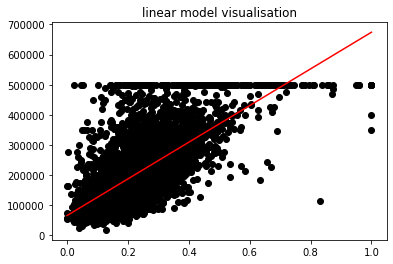
\includegraphics[width=0.5\textwidth]{4.png}
    \caption{\centering MLR grafik}
\end{figure}      
\subsection{Polinomijalna linearna regresija (PLR)}
Dobijen izlaz 4. za primenjen algoritam PLR modela je takav da mu je MSE: $0.0$, RMSE: $0.0$, R2 score: ~$-0.54$.
\begin{lstlisting}[caption=\centering PLR]
    polynomial_regression
    mean square error: 0.0
    root mean square error: 0.0
    
    R2 score: -0.5451445244202564
\end{lstlisting}
Na slici 4. je prikazan grafik ishodujuće regresije, stepena 3, sagledajući, po mom mišljenju bolji za vizuelizaciju, feature \verb|households|. Većina ostalih features-a ima sličan oblik pozicija uzoraka.

\begin{figure}[h!]
    \centering
    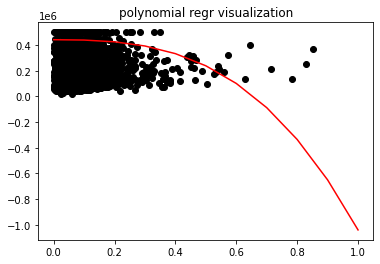
\includegraphics[width=0.5\textwidth]{3.png}
    \caption{\centering PLR grafik}
\end{figure}      
\subsection{Regresija stabla odlučivanja}
Dobijen izlaz 5. za primenjen algoritam  modela je takav da mu je MSE: $0.0$, RMSE: $0.0$, R2 score: ~$-0.63$.
\begin{lstlisting}[caption=\centering Stabla odlučivanja]
decision tree
mean square error: 0.0
root mean square error: 0.0
R2 score: 0.6309696611415031
\end{lstlisting}

Za najbolji moguć sastav hiperparametara:
\begin{itemize}
    \item \verb|splitter == 'best'|,
    \item \verb|max_depth == 5|,
    \item \verb|min_samples_leaf == 1|,
    \item \verb|min_weight_fraction_leaf == 0.1|,
    \item \verb|max_features == None|,
    \item \verb|max_leaf_nodes == None|.
\end{itemize}
dobijen je ishodujući rezultat na izlazu 6. gde mere važe za MSE: $6567139517.78$, RMSE: $81037.89$, R2 score: ~$0.51$.
\begin{lstlisting}[caption=\centering Stabla odlučivanja sa optimizacijom hiperparametrima]
decision tree with hyperparameter optimization
mean square error: 6567139517.78
root mean square error: 81037.89
R2 score: 0.5059771880336792
best params after grid search: 
{'max_depth': 5, 'max_features': None, 'max_leaf_nodes': None, 'min_samples_leaf': 1, 'min_weight_fraction_leaf': 0.1, 'splitter': 'best'}
\end{lstlisting}

\subsection{Regresija slučajne šume}
Dobijen izlaz 7. za primenjen algoritam  modela je takav da mu je MSE: $0.0$, RMSE: $0.0$, R2 score: ~$-0.79$.

\begin{lstlisting}[caption=\centering Slučajne šume]
random forest
mean square error: 0.0
root mean square error: 0.0
R2 score: 0.7906854214130685
\end{lstlisting}
Za najbolji moguć sastav hiperparametara:
\begin{itemize}
    \item \verb|n_estimators == 150|,
    \item \verb|max_depth == 9|,
    \item \verb|min_samples_leaf == 1|,
    \item \verb|max_features == None|,
    \item \verb|max_leaf_nodes == 9|.
\end{itemize}
dobijen je ishodujući rezultat na izlazu 8. gde mere važe za MSE: $5766173566.8$, RMSE: $75935.32$, R2 score: ~$0.57$.

\begin{lstlisting}[caption=\centering Slučajne šume sa optimizacijom hiperparametrima]
Random Forest with hyperparameter optimization
mean square error: 5766173566.8
root mean square error: 75935.32
R2 score: 0.5662310398546941
best params after grid search: 
{'max_depth': 9, 'max_features': None, 'max_leaf_nodes': 9, 'n_estimators': 150}
\end{lstlisting}

\subsection{Regresija potpornim vektorima (SVR)}
Dobijen izlaz 9. za primenjen algoritam  modela je takav da mu je MSE: $0.0$, RMSE: $0.0$, R2 score: ~$-0.05$.

\begin{lstlisting}[caption=\centering SVR]
svr
mean square error: 0.0
root mean square error: 0.0
R2 score: -0.045590393753930814
\end{lstlisting}

Za najbolji moguć sastav hiperparametara:
\begin{itemize}
    \item \verb|C == 100|,
    \item \verb|gamma == 1|,
    \item \verb|kernel == 'poly'|.
\end{itemize}
dobijen je ishodujući rezultat na izlazu 10. gde mere važe za MSE: $8730005894.59$, RMSE: $93434.5$, R2 score: ~$0.34$.

\begin{lstlisting}[caption=\centering SVR sa optimizacijom hiperparametrima]
Support vector regression with hyperparameter optimization
mean square error: 8730005894.59
root mean square error: 93434.5
R2 score: 0.3432723564267346
best params after grid search: 
{'C': 100, 'gamma': 1, 'kernel': 'poly'}
\end{lstlisting}

%%%%%%%%%%%%%%%%%%%%%%%%%%%%%%%%

\newpage
\section{Zaključak}
Predstavljeni slučajevi tačnosti za svaki model regresije na tabeli 1. može se uočiti da je najbolji model \textbf{MLR}. Sa druge strane, je najgori slučajne šume. 

I moguće je uočiti da je pospešujuć efekat optimizacija hiperparametrima nad modelima nad kojima je bio primenjivan.
\begin{table}[h]
    \centering
    \begin{tabular}{|r|c|c|c|}
    \hline
    \textbf{Klasifikator} & \textbf{MSE} & \textbf{RMSE} & \textbf{R2 score}\\
    \hline
    SLR nad \verb|median_income| & 274334668.63 & 85289.71 & 0.46\\
    \hline
    MLR & 5180413707.33 & 71975.09 & 0.61 \\
    \hline
    PLR & 0.0 & 0.0 & -0.54 \\
    \hline 
    Stablo odlučivanja & 0.0 & 0.0 & -0.63 \\
    \hline 
    Stablo odlučivanja sa optimizacijom hiperparametrima & 567139517.78 &
    81037.89 & 0.51 \\
    \hline
    Slučajne šume & 0.0 & 0.0 & -0.79 \\
    \hline
    Slučajne šume sa optimizacijom hiperparametrima & 766173566.8 & 75935.32 & 0.57 \\
    \hline
    SVR & 0.0 & 0.0 & -0.05 \\
    \hline
    SVR sa optimizacijom hiperparametrima & 730005894.59 & 93434.5 &0.34 \\
    \hline
    \end{tabular}
    \caption{Prikaz tačnosti klasifikatora sa i bez primene optimizacije hiperparametara.} 
\end{table}

%%%%%%%%%%%%%%%%%%%%%%%%%%%%%%%%%%%%%%%%%%%%%%%%%%%%

% \cite{humancpu}

% \subsection{\normalsize{Pogled na pojmove inteligencije, znanja, ljudske imitacije}}
% \subsubsection{\normalsize{Istorija temelja veštačke inteligencije}}



% \begin{enumerate}
    % \item [3.]{\textbf{Da li uticaj misli tradicionalnog zapadnog sveta obazirale su se nad pitanjem odnosa tela i uma kao: 
    % bla bla

    % \item[5.] {\textbf{Moja lična zahtevanja oko inteligencije računarkog softvera.}}
    % bla bla

% \end{enumerate}
\newpage

\begin{thebibliography}{1}
    \bibitem{dataset}
    California Housing (EDA + linear regression), \url{https://www.kaggle.com/code/mohamedkhaledelsafty/california-housing-eda-linear-regression}, Datum poslednjeg pristupa: \today
    \bibitem{mojRad}
    Ž. Simić, (2024), ``Teorijski izveštaj o regresionim algoritmima sa nadgledanim učenjem'', Univerzitet u Kragujevcu
    \bibitem{pandasDF}
    DataFrame, \url{https://pandas.pydata.org/docs/reference/frame.html}, Datum poslednjeg pristupa: \today
    \bibitem{labelEncoding}
    sklearn.preprocessing.LabelEncoder, \url{https://scikit-learn.org/stable/modules/generated/sklearn.preprocessing.LabelEncoder.html}, Datum poslednjeg pristupa: \today
    \bibitem{scaleDist}
    When should I use StandardScaler and when MinMaxScaler?, \url{https://scikit-learn.org/stable/modules/generated/sklearn.preprocessing.LabelEncoder.html}, Datum poslednjeg pristupa: \today
    \bibitem{train_test_split}
    {sklearn.model\_selection.train\_test\_split}, \url{https://scikit-learn.org/stable/modules/generated/sklearn.model_selection.train_test_split.html}, Datum poslednjeg pristupa: \today
    \bibitem{pairplot}
    seaborn.pairplot, \url{https://seaborn.pydata.org/generated/seaborn.pairplot.html}, Datum poslednjeg pristupa: \today
    \bibitem{displot}
    seaborn.displot, \url{https://seaborn.pydata.org/generated/seaborn.displot.html}, Datum poslednjeg pristupa: \today
    \bibitem{LR}
    sklearn.linear\_model.LogisticRegression, \url{https://scikit-learn.org/stable/modules/generated/sklearn.linear\_model.LogisticRegression.html#sklearn.linear\_model.LogisticRegression}, Datum poslednjeg pristupa: \today
    \bibitem{plr}
    sklearn.preprocessing.PolynomialFeatures, \url{https://scikit-learn.org/stable/modules/generated/sklearn.preprocessing.PolynomialFeatures.html}, Datum poslednjeg pristupa: \today
    \bibitem{DTR}
    sklearn.tree.DecisionTreeRegressor, \url{https://scikit-learn.org/stable/modules/generated/sklearn.tree.DecisionTreeRegressor.html#sklearn.tree.DecisionTreeRegressor}, Datum poslednjeg pristupa: \today
    \bibitem{GridSearchCV}
    sklearn.model\_selection.GridSearchCV, \url{https://scikit-learn.org/stable/modules/generated/sklearn.model\_selection.GridSearchCV.html}, Datum poslednjeg pristupa: \today
    \bibitem{RFR}
    sklearn.ensemble.RandomForestRegressor, \url{https://scikit-learn.org/stable/modules/generated/sklearn.ensemble.RandomForestRegressor.html}, Datum poslednjeg pristupa: \today
    \bibitem{SVR}
    sklearn.svm.SVR, \url{https://scikit-learn.org/stable/modules/generated/sklearn.svm.SVR.html#sklearn.svm.SVR}, Datum poslednjeg pristupa: \today
    

\end{thebibliography}

% \title{Seminarski rad}
% \subtitle{Razvoj i oblasti veštačke inteligencije}
% \date{}
% \author{}

% ja ne razumem nista

% {Seminarski rad} \hfill ovo radi \hfill student: Željko Simić

% \hfill what's up?
% \maketitle


% eyo


\end{document}